%///////////////////////////////////////////////////////////////////////////////
% <file
%   repository_path  = "$Source: /pub/cvsprojects/nucleo/web/home/modules/wn_matrix/doc/tex/arrow.tex,v $"
%   revision         = "$Revision: 1.5 $"
%   date             = "$Date: 2009/04/25 03:42:35 $"
%   tag              = "$Name: wn_matrix-0-24 $"
%   template_version = "cp_template.0.12"
% >
%
% <license>
%   See the README_module.xml file for this module for copyright and license
%   information.
% </license>

%   <description>
%     <abstract>
%       This is the Webnucleo Report for the arrow solver in the wn_matrix
%       Module.
%     </abstract>
%     <keywords>
%       wn_matrix Module, webnucleo report
%     </keywords>
%   </description>
%
%   <authors>
%     <current>
%       <author userid="mbradle" start_date="2009/02/26" />
%     </current>
%     <previous>
%     </previous>
%   </authors>
%
%   <compatibility>
%     TeX (Web2C 7.4.5) 3.14159 kpathsea version 3.4.5
%   </compatibility>
%
% </file>
%///////////////////////////////////////////////////////////////////////////////
%
% This is a sample LaTeX input file.  (Version of 9 April 1986)
%
% A '%' character causes TeX to ignore all remaining text on the line,
% and is used for comments like this one.

\documentclass{article}    % Specifies the document style.

\usepackage{hyperref}
\usepackage{graphicx}

                           % The preamble begins here.
\title{Webnucleo Technical Report: The Arrow Solver in the wn\_matrix Module}  

\author{Bradley S. Meyer}
%\date{December 12, 1984}   % Deleting this command produces today's date.

\begin{document}           % End of preamble and beginning of text.

\maketitle                 % Produces the title.

As of version 0.8 of wn\_matrix, there is a Gaussian elimination solver for
an ``arrow'' type matrix.  An arrow-type matrix is one for which the non-zero
elements form a band along the diagonal and two wings along the far right
and bottom of the matrix.  

\section{The WnMatrix\_\_Arrow Structure}

The form of an arrow matrix is shown schematically in Fig.
\ref{fig:arrow}.  The matrix has $N$ rows, therefore, in dense form it has
$N \times N$ elements.  The arrow matrix has band width $n$ and wing width
$m$.  The arrow matrix comprises four submatrices, as shown in
Fig. \ref{fig:arrow}.  The $a$ matrix has $N - m$ rows and $n$ columns.
The row index of $a$ corresponds to the row index of the parent matrix
while the column index gives the position relative to the diagonal.  Matrix
elements in the central band
farthest from the diagonal are $m_b = (n - 1)/2$ columns away from the
diagonal.  The $b$ matrix is one of the wings of the arrow.  It has $m$
rows corresponding to the columns beyond the column $N - m$ and $N - m$
columns corresponding to the row of the element.  The $c$ matrix has
$m$ rows corresponding to rows beyond the row $N - m$ in the parent matrix
and $N - m$ columns corresponding to the columns in the parent matrix.
Finally, the $d$ matrix is an $m \times m$ matrix with indices corresponding
to the most rightward and bottom elements in the parent matrix.

\begin{figure}[thp]
\centering
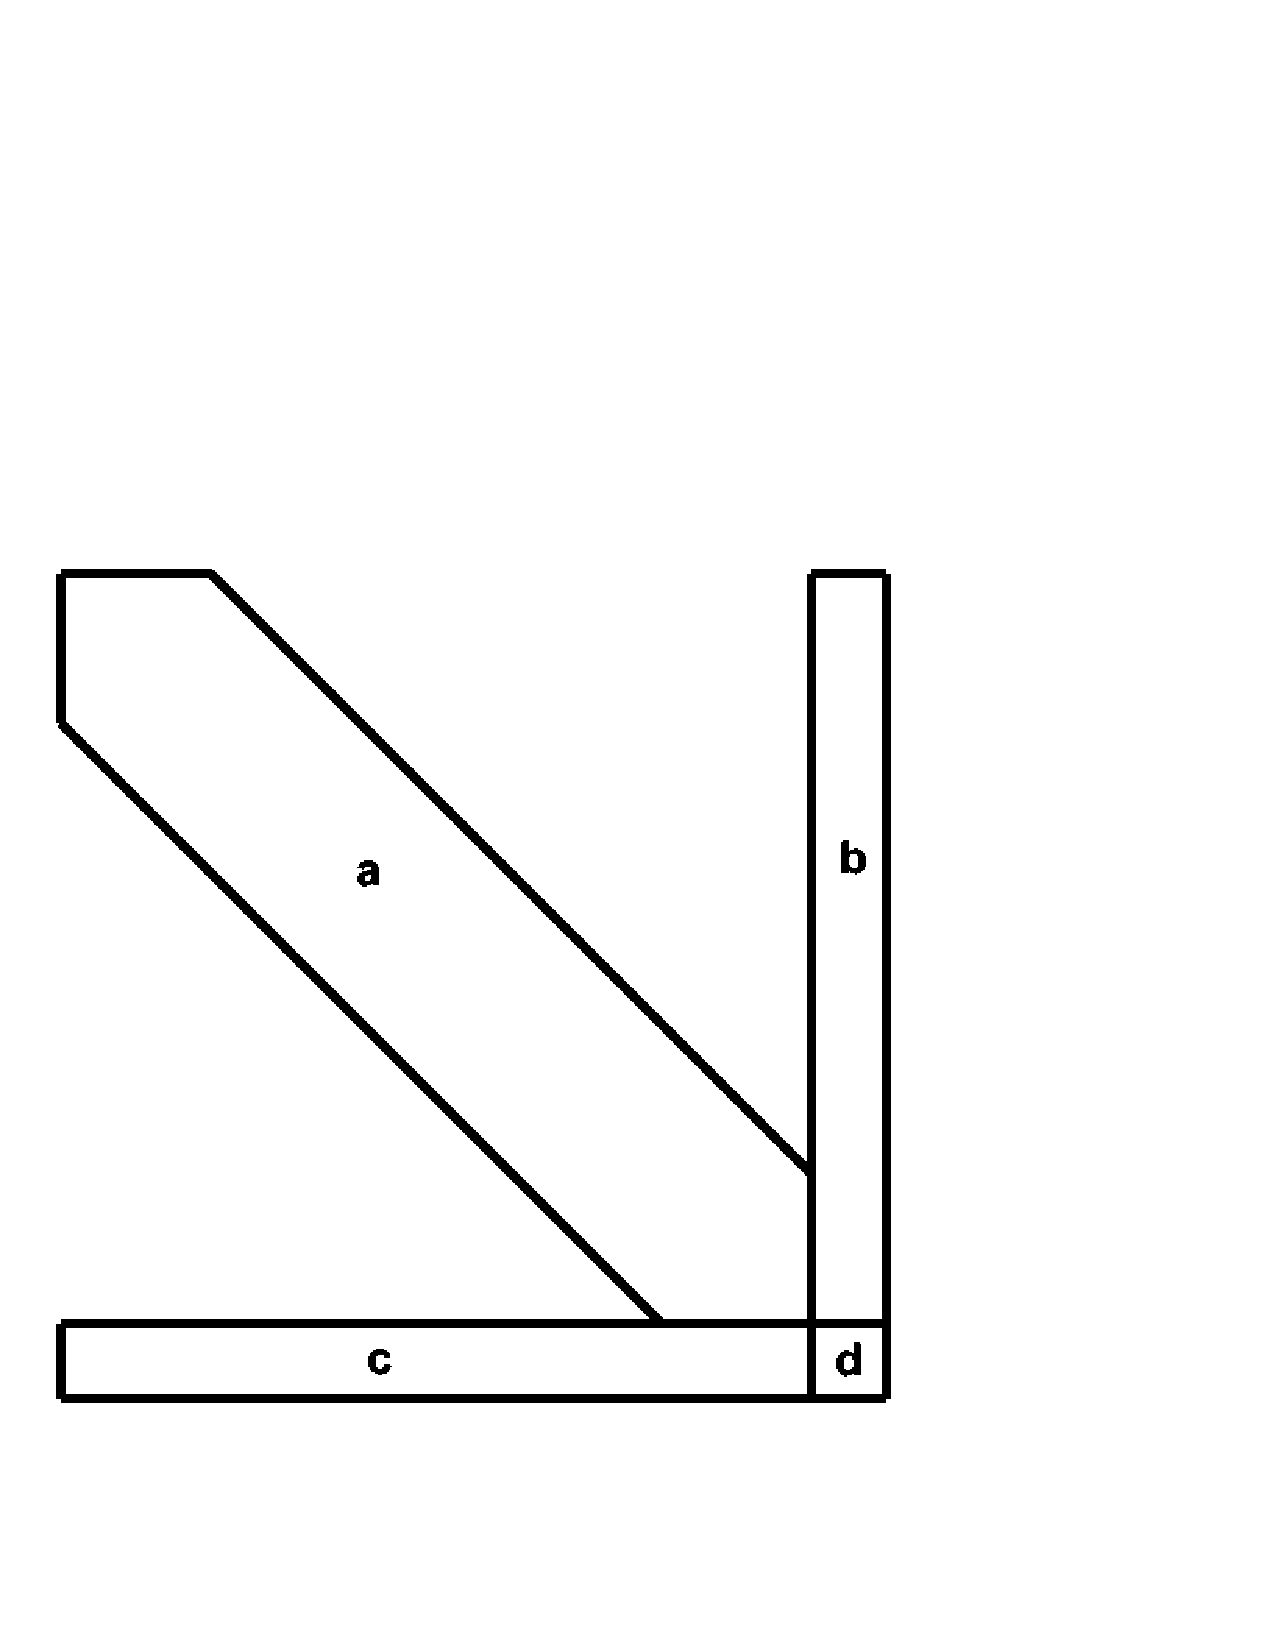
\includegraphics[width=2in]{figures/matrix1.pdf}
\caption{Arrow matrix.}
\label{fig:arrow}
\end{figure}

The mapping between an element in the parent matrix $M(i,j)$ at row $i$ and
column $j$ and the corresponding element in the arrow matrix is determined
as follows.  If $i \leq N - m$ and
$j \leq N - m$, then $a(i, m_b + 1 - i + j) = 
M(i,j)$.  If $i \leq N - m$ and $j > N - m$, then $b(j - N + m, i) = M(i,j)$.
If $i > N - m$ and $j \leq N - m$, then $c(i - N + m, j) = M(i,j)$.  Finally,
if $i > N - m$ and $j > N - m$, then $d(i - N + m, j - N + m) = M(i,j)$.
The above mappings assume 1-based indexing.  Notice that the full range
on the second index of the $a$ matrix can put the index outside the
parent matrix.  This array must therefore be checked to ensure it remains
in bounds.  It should be clear that the arrow matrix form requires storage
of $(N - m) * (n + 2 m) + m^2$ elements.  If $n,m << N$, the arrow format
can result in substantial storage savings over the dense form.

The data for the arrow matrix are stored in a WnMatrix\_\_Arrow structure,
which is obtained from a WnMatrix structure by the API routine with
prototype\\
\\
WnMatrix\_\_Arrow *\\
WnMatrix\_\_getArrow( WnMatrix *p\_matrix, size\_t i\_wing).\\
\\
Here i\_wing is the desired wing width for the arrow matrix (the quantity $m$).
The routine determines the appropriate band width from the parent matrix.
Diagnostics on the arrow matrix are available from the API routines\\
\\
size\_t\\
WnMatrix\_\_Arrow\_\_getNumberOfRows( WnMatrix\_\_Arrow * p\_arrow\_matrix ),\\
\\
which returns $N$, the number of rows,\\
\\
size\_t\\
WnMatrix\_\_Arrow\_\_getWingWidth( WnMatrix\_\_Arrow * p\_arrow\_matrix ),\\
\\
which returns $m$, the wing width, and\\
\\
size\_t\\
WnMatrix\_\_Arrow\_\_getBandWidth( WnMatrix\_\_Arrow * p\_arrow\_matrix ),\\
\\
which returns $n$, the band width.

\begin{figure}[thp]
\centering
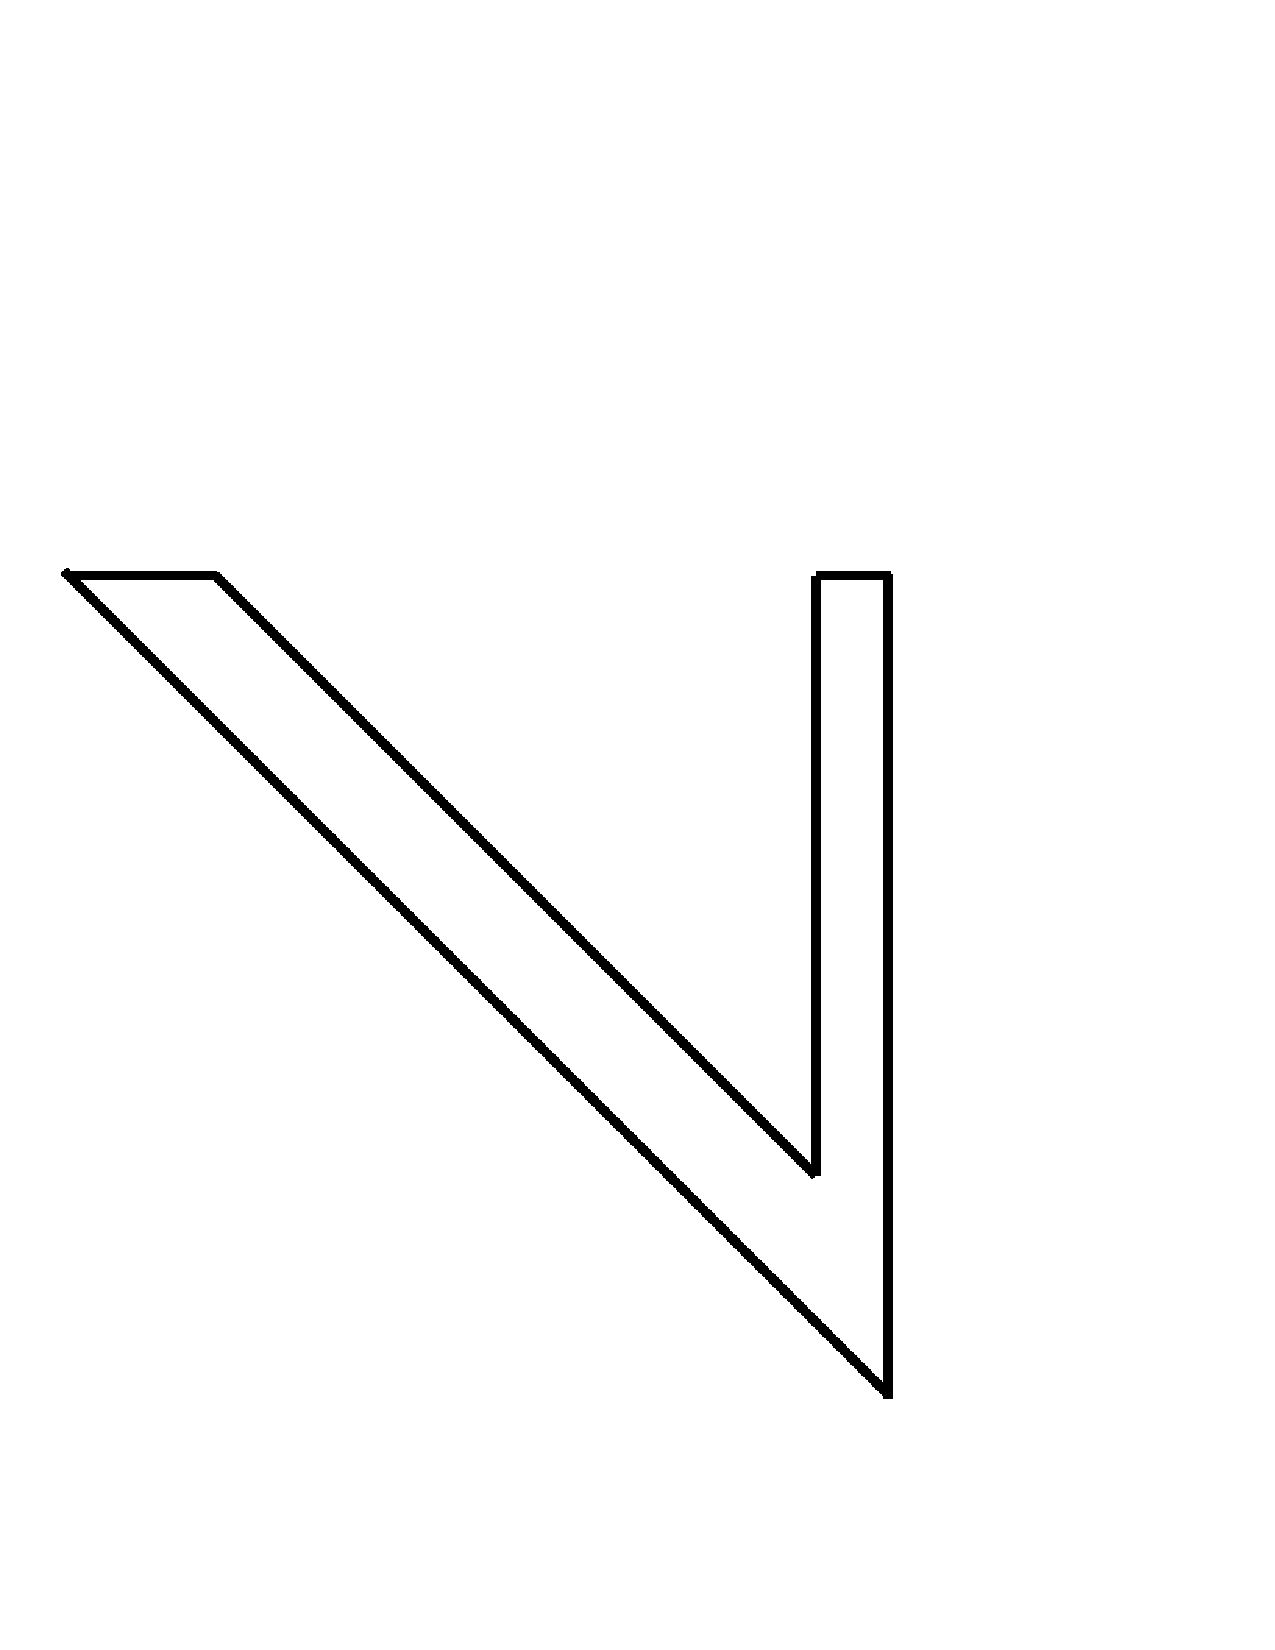
\includegraphics[width=2in]{figures/matrix2.pdf}
\caption{Arrow matrix after Gaussian elimination.}
\label{fig:eliminated}
\end{figure}

\section{Solving an Arrow Matrix Equation}

We suppose now that we have the matrix equation $A x = b$.  If the matrix
A is stored as a WnMatrix\_\_Arrow matrix p\_arrow\_matrix and the
right-hand-side vector $b$ is stored as a gsl vector pointed to by p\_rhs,
the user may find the solution vector p\_solution from an API routine
as:\\
\\
p\_solution = WnMatrix\_\_Arrow\_\_solve( p\_arrow\_matrix, p\_rhs ).\\
\\
p\_solution is another gsl vector.  The routine solves the matrix by
Gaussian elimination.  Through row operations, the routine reduces the
matrix to the form shown in Fig. \ref{fig:eliminated}.  Simultaneous
operations change the rhs vector.  From this form,
simple backsubstitution gives the solution vector.  The arrow matrix
and the rhs vector returned from WnMatrix\_\_Arrow are those after
the row operations.  This permits diagnostics on the solution.  
For example, after the solution is obtained, the user can get a
WnMatrix form for the arrow from the API routine\\
\\
p\_solved\_matrix = WnMatrix\_\_Arrow\_\_getWnMatrix( p\_arrow\_matrix )\\
\\
which may be studied or output to text with other API routines.  Since
the solver modifies the input matrix and rhs vector, the user should
make copies of those prior to solving the matrix equation if he or
she requires those later. 
Once the user is done with the arrow matrix, he or she should
free it with the API routine WnMatrix\_\_Arrow\_\_free().

\end{document}

